\subsection{Football Player Tiers using Transfer Data}\label{ssec:transfer}

Our objective in this data analysis is to investigate 
whether it is possible to classify football players into tiers
using only transfer data to indicate their status within the football community.
We used the publicly available dataset that contains the top 250 transfers 
(in terms of price) from 2000-2018 on
\href{https://www.kaggle.com/vardan95ghazaryan/top-250-football-transfers-from-2000-to-2018}{Kaggle}
\footnote{https://www.kaggle.com/vardan95ghazaryan/top-250-football-transfers-from-2000-to-2018}. 
As an example, Cristiano Ronaldo and Kylian Mbapp\'e are two very highly regarded 
football talents and, as we will see in Section~\ref{sssec:transfer-data}, 
are found in this dataset.
We are interested in seeing if and how SOM can be used to stratify 
these transfers differently from other players. 

\subsubsection{Data Description}\label{sssec:transfer-data}

In this section, we will describe the dataset that we used
and the cleaning process.
The original dataset has 4700 observations and the following 10 features: 
player age, name, playing position, club/league transferred to/from, season played,
estimated market value, and transfer fee.
After removing the rows with missing values, we have a total of 3440 observations. 
We change the unit of market value and transfer fee into 1 million. 
We clean the data entries for the leagues because some leagues were represented
with non-unique names, and some leagues should have been further 
differentiated based on the club. 
More detail can be found in the code\footnote{https://github.com/jyzhang27/STATS305C-SOM}. 
There are a total of 64 unique leagues and 467 unique clubs, 
which is overly granular for our application. 
Hence, we simplify each row by changing the league type
into one of six categories that they transferred to and from.
The categories are based on geographical regions and league ratings:

\begin{itemize}
    \item Big5 (count: 5):
        England's Premier League, 
        Italy's Serie A, 
        France's Ligue 1, 
        Spain's LaLiga, 
        and Germany's Bundesliga.
    \item Europe (count: 20): 
        All other European top-flight leagues 
        (e.g. the Eredivisie of the Netherlands or 
        the S\"{u}per Lig of Turkey).
    \item Asia Africa (count: 10): 
        The top-flight leagues in Asia or Africa
        (e.g. the J1 league of Japan).
    \item Americas (count: 9): 
        The top-flight leagues in North and South America
        (e.g. the Liga MX of Mexico).
    \item Big5 B (count: 13): 
        The lower-division leagues in the Big5 countries.
    \item Other B (count: 7): All other lower-division leagues.
\end{itemize}

Finally, we categorize the 13 total player positions into 4 main categories: 
defense, midfield, forward, and goalkeeper. 

After applying these changes to the data,
we gather some quick summaries of our data to get some insight.

\begin{table}[H]
    \centering 
    \begin{tabular}{|l|llllll|} 
    \hline 
       & Min. & 1st Qu. & Median  &  Mean& 3rd Qu. &Max. \\  \hline 
       Market Value & 0.05 &  3.5 &  6 &  8.622 & 10 & 120 \\ 
       Transfer Fee &   1.5 &   5 &   7.5 &  10.65 &  12  &222  \\ \hline 
    \end{tabular}
    \caption{Summary of market value and transfer fee in the data.}
    \label{tab:transfer-quick-summary}
\end{table}

Table~\ref{tab:transfer-quick-summary} displays a quick summary of 
market value and transfer fee, which
shows that they seem to have some extreme outliers 
that are large.
This indicates a couple very expensive superstar players,
and upon inspection, the three names associated with the highest market value are
Kylian Mbapp\'e, Neymar, and Cristiano Ronaldo.

\begin{table}[H]
    \centering
    \begin{tabular}{|l|llllll|} 
    \hline 
          & Big5    &  Europe &   Americas & Asia Africa & Big5 B  &  Other B \\ \hline 
        From &   2039  &756 &205 & 61   &366 &   13 \\
        To &  2547 &   560 &  56  & 176 &   100 & 1 \\ \hline 
    \end{tabular}
    \caption{Counts of the different categories of leagues (each column) that transfers went to and from.}
    \label{tab:transfer-counts-leagues}
\end{table}

Table~\ref{tab:transfer-counts-leagues} is the league type breakdown. 
As expected, the most expensive transfers to and from occur in the Big5 leagues 
and in Europe, in general.

For the purposes of running the SOM algorithm, 
we remove some of the original features in the dataset. 
The features we will consider are:
age, market value, transfer fee, position type
leagues transferred to, and leagues transferred from.
In addition, the numerical features will be standardized to mean 0 and standard deviation 1 
when running the algorithm because SOM is not scale-invariant.

\subsubsection{Hierarchical Clustering Analysis}\label{sssec:transfer-hc}

\begin{figure}[t]
    \centering
    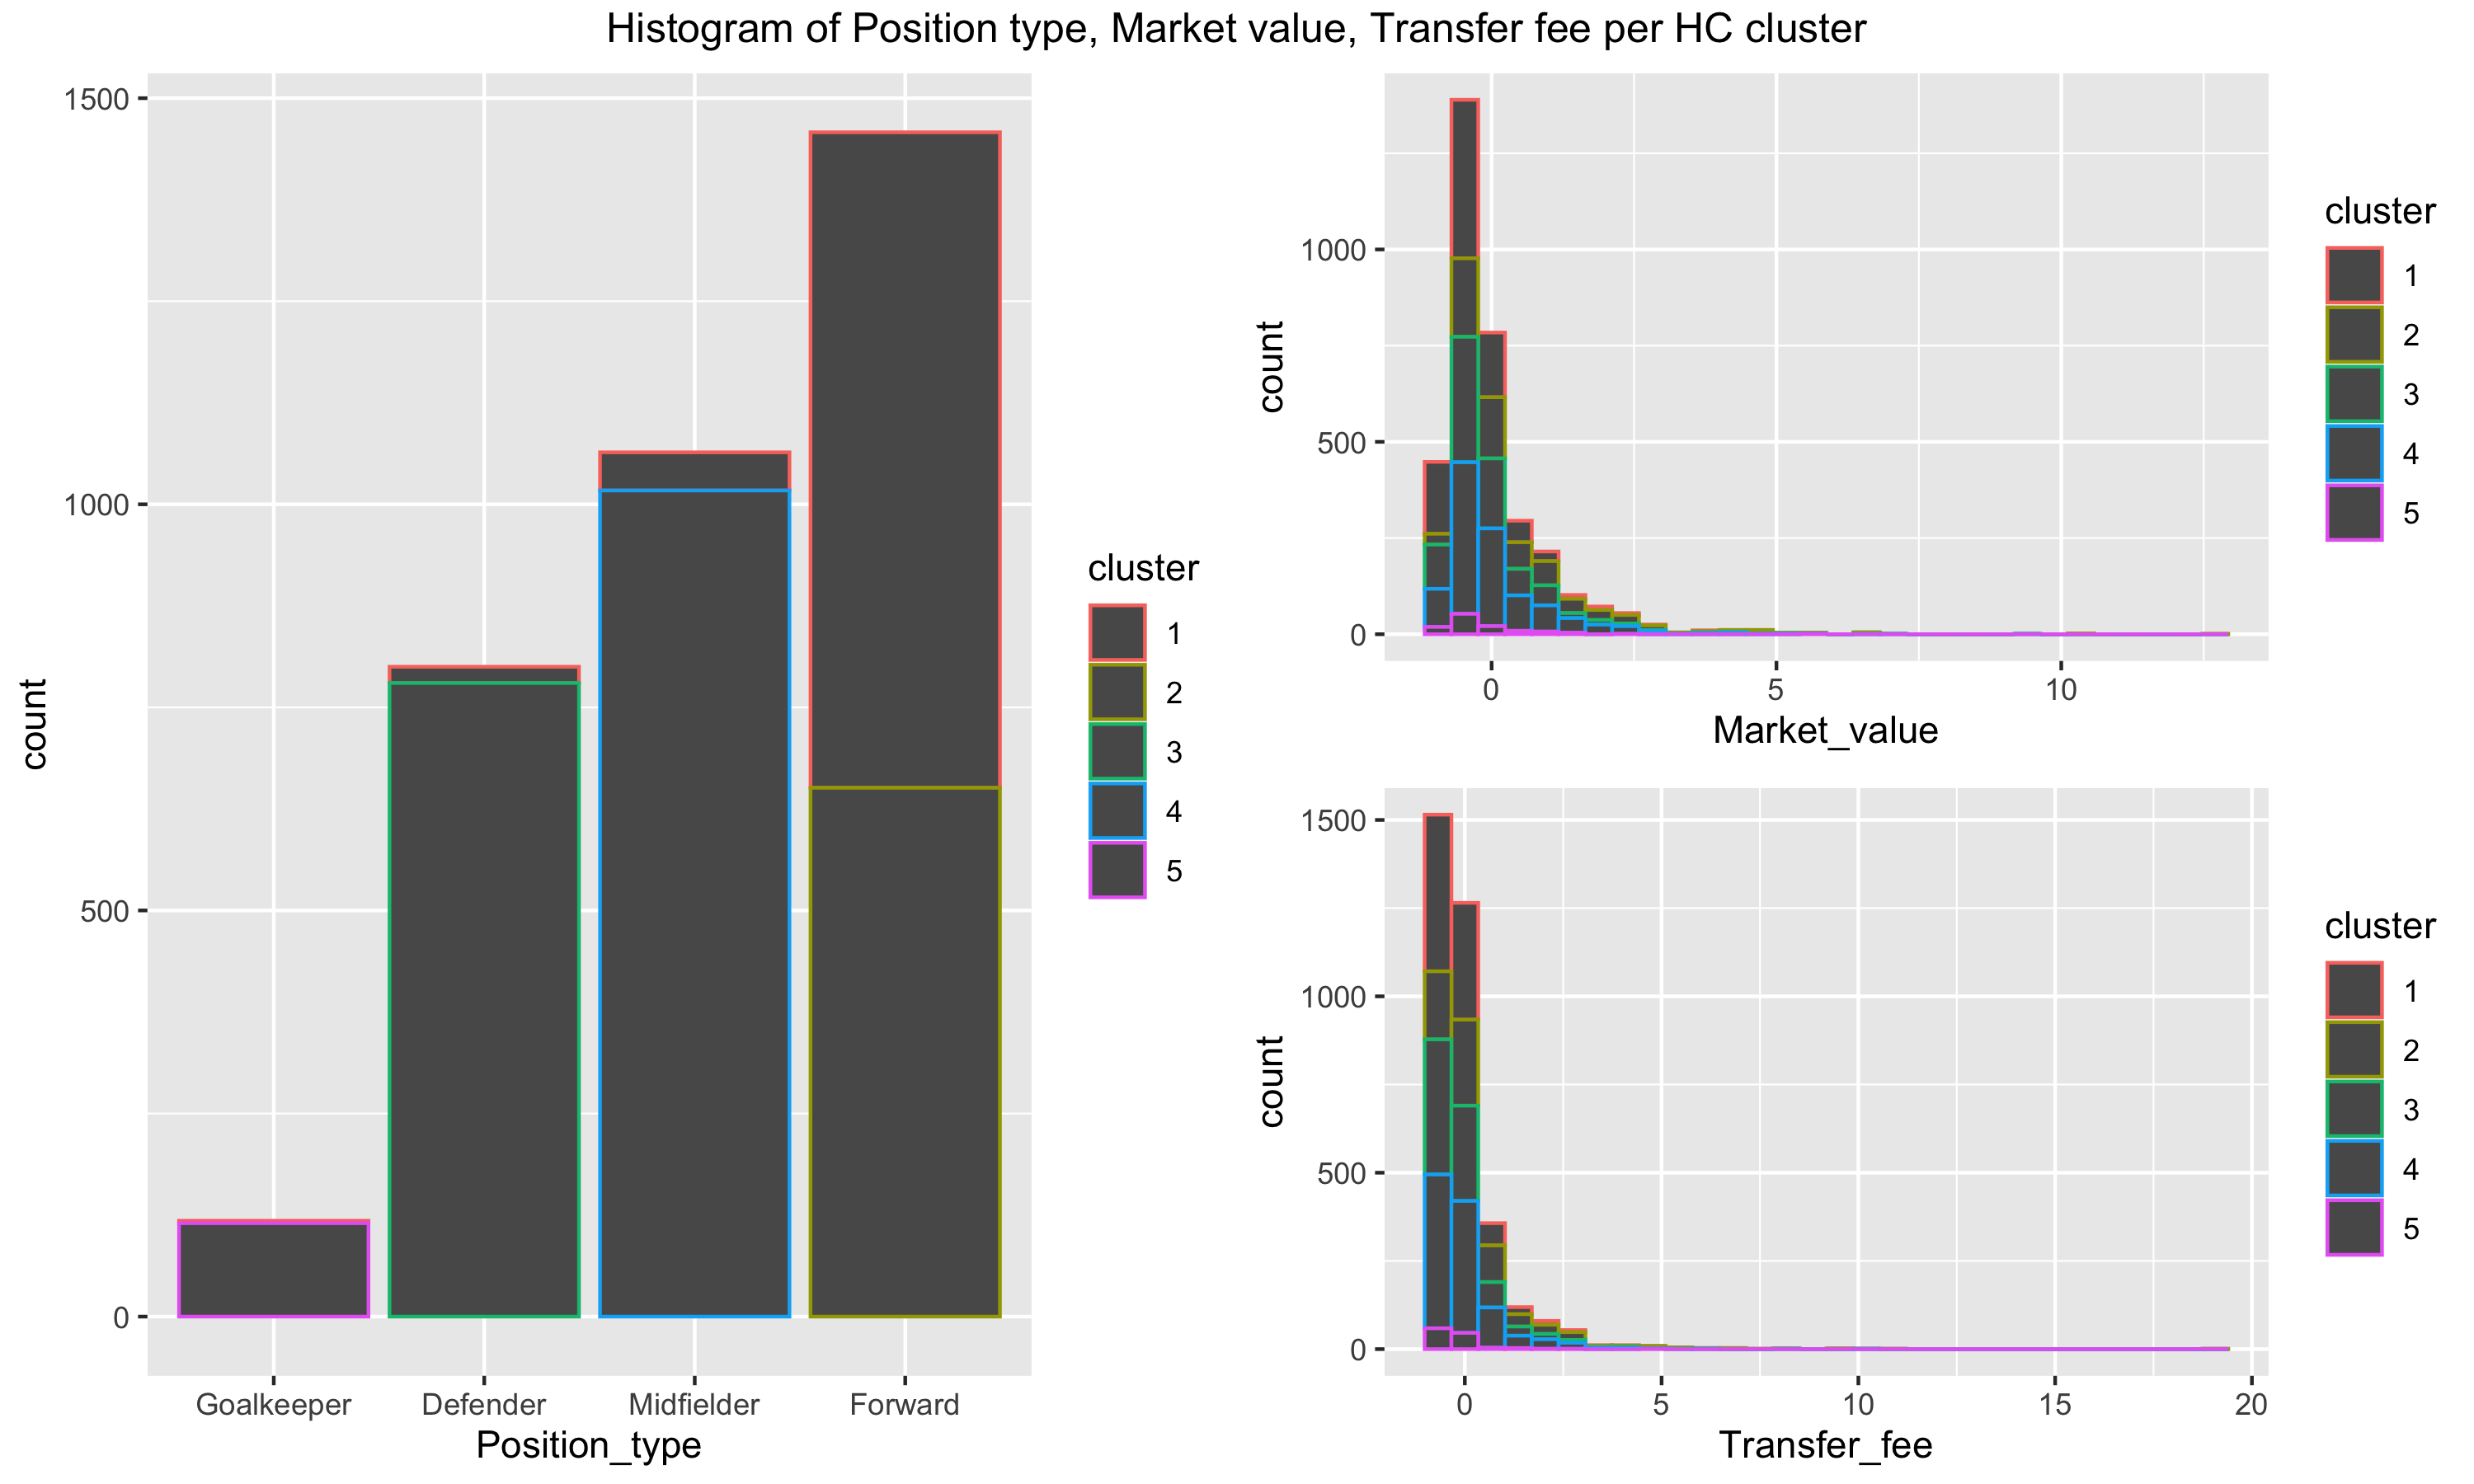
\includegraphics[width=\textwidth]{../figs/transfer_hc_ppmvtf.png}
    \caption{Distribution of player position, 
             market value, and transfer fee for 
             each of the 5 clusters defined by hierarchical clustering.}
    \label{fig:hc-ppmvtf}
\end{figure}

Before running SOM, we first use hierarchical clustering
to further motivate the need for a more sophisticated model.
We apply hierarchical clustering directly to the dataset with 5 clusters.
Figure~\ref{fig:hc-ppmvtf} shows the distribution of player position,
market value, and transfer fee, for each of the 5 clusters defined by hierarchical clustering.
It shows a strong stratification by player position 
as we see that each position type is dominated by a different cluster,
with the exception of forward position, which is dominated by clusters 1 and 2 equally.
The distribution of market value and transfer fee show that
unlike the position distribution, none of the clusters
dominate any region of these values with the exception of cluster 5 that 
dominates for large values; otherwise, we see relatively equal representation
across all moderate values.
This indicates that hierarchical clustering seemed to naively cluster
predominantly based on the position types of players without using 
the features that we wished to use to distinguish these players,
i.e.\ market value and transfer fee.
In this sense, hierarchical clustering does not give us any more insight
on categorizing players into tiers than simply stratifying them based on their position.
We will soon see, however, that applying hierarchical clustering to the \emph{U-matrix},
or the distance matrix for the codebook vectors,
gives us entirely different results that are more interesting.

\subsubsection{SOM Analysis}

\begin{figure}[t]
    \centering
    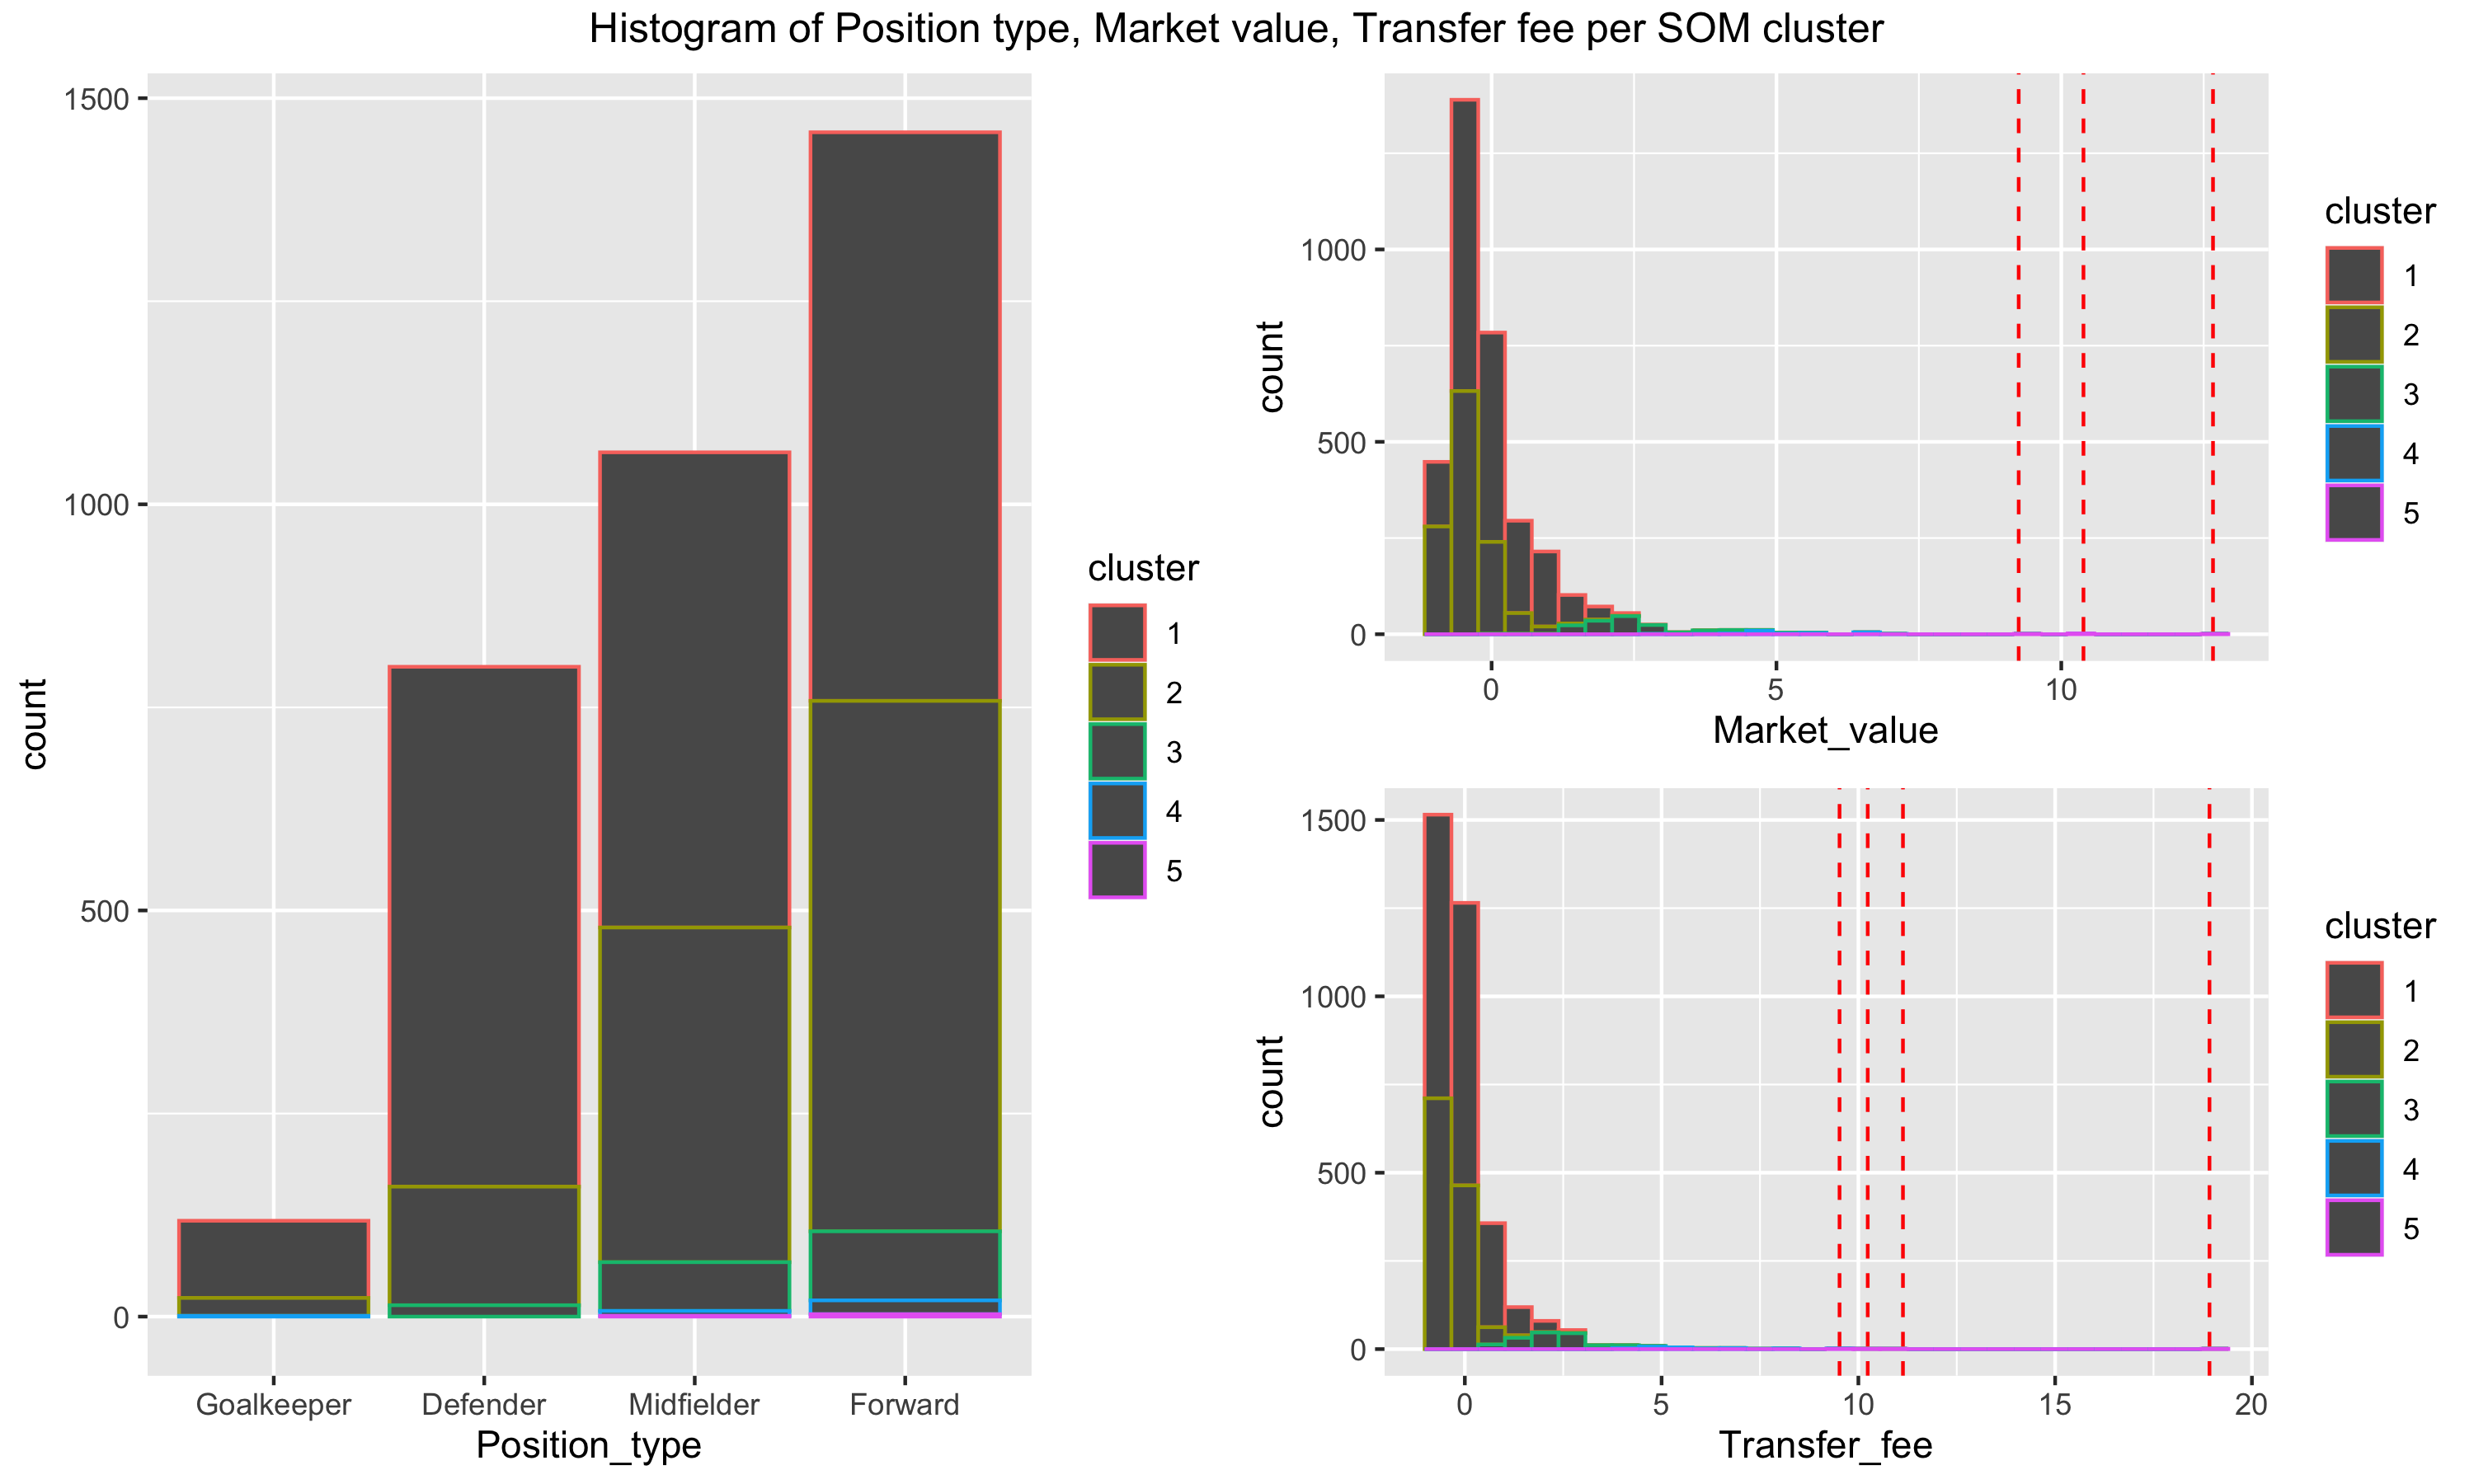
\includegraphics[width=\textwidth]{../figs/transfer_som_ppmvtf.png}
    \caption{Distribution of player position, 
             market value, and transfer fee for 
             each of the 5 clusters defined by hierarchical clustering
             on the U-matrix from SOM.
             The red dashed lines indicate the exact values from samples in cluster 5.}
    \label{fig:som-ppmvtf}
\end{figure}

We apply the SOM algorithm in batch mode with 500 total iterations, 
default learning-rate $\alpha(t)$ that decreases linearly from 0.05 to 0.01 per iteration,
a hexagonal grid size $20 \times 15$,
and the Gaussian neighborhood function.
Figure~\ref{fig:som-ppmvtf} shows the analogous distribution of
player position, market value, and transfer fee for each of the 5 clusters
defined by running hierarchical clustering on the U-matrix from SOM.
We immediately see the distributions are reversed in the sense that
the position distribution now has relatively equal representation across all clusters
while market value and transfer fee are better stratified with
cluster 5 dominating values greater than 5, 
cluster 4 dominating values between 3 and 5,
cluster 3 dominating values between 1.5 and 3,
and clusters 1 and 2 dominating the lowest values.
This shows that SOM learns the similarity of our sample points
that is far more refined than a simple dissimilarity matrix
used in the naive hierarchical clustering method in Section~\ref{sssec:transfer-hc},
which supports our claim in Section~\ref{sec:introduction}.

\begin{figure}[t]
    \centering
    \begin{subfigure}[b]{0.4\textwidth}
        \centering
        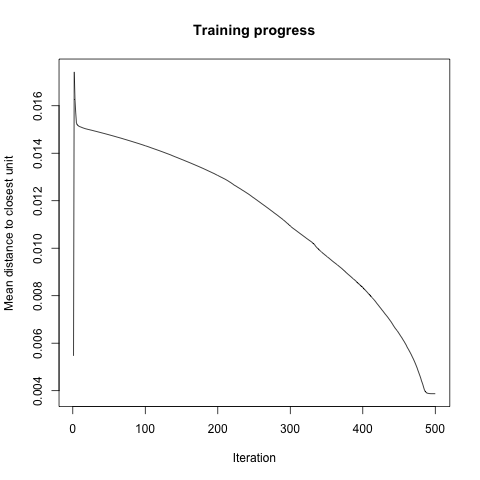
\includegraphics[width=\textwidth]{../figs/transfer_training.png}
        \caption{SOM training plot of mean distance to closest unit over the iterations.}
        \label{fig:transfer-training}
    \end{subfigure}
    \begin{subfigure}[b]{0.4\textwidth}
        \centering
        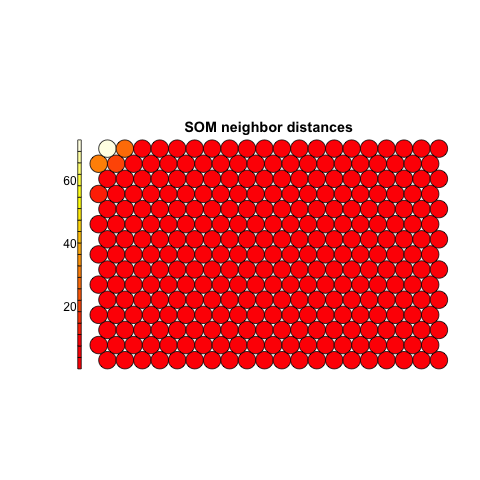
\includegraphics[width=\textwidth]{../figs/transfer_U.png}
        \caption{SOM neighbor distance.}
        \label{fig:transfer-neighbor-dist}
    \end{subfigure}
    \begin{subfigure}[b]{0.45\textwidth}
        \centering
        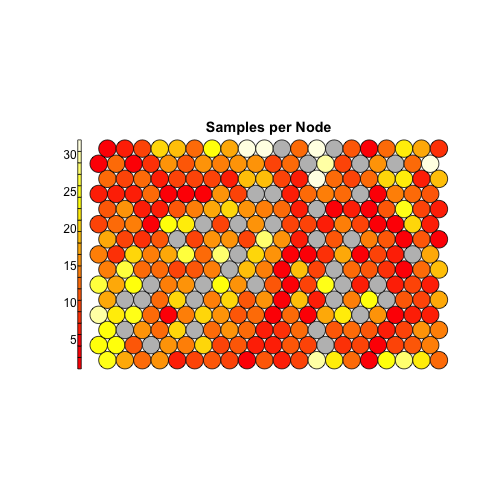
\includegraphics[width=\textwidth]{../figs/transfer_node_samples.png}
        \caption{SOM number of variables in each node.}
        \label{fig:transfer-nvar}
    \end{subfigure}
    \begin{subfigure}[b]{0.45\textwidth}
        \centering
        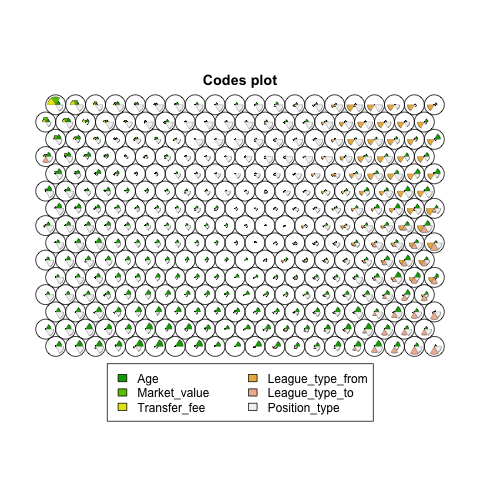
\includegraphics[width=\textwidth]{../figs/transfer_codebook.png}
        \caption{SOM codebook vectors.}
        \label{fig:transfer-codebooks}
    \end{subfigure}
    \caption{}
    \label{fig:transferplots}
\end{figure}

Figure~\ref{fig:transfer-training} serves as a visual check 
that the algorithm converged and 
Figure~\ref{fig:transfer-nvar} shows that we picked a suitable grid size
since we see a large number of nodes with 10-20 samples.
We can view the plot of the codebook vectors in Figure~\ref{fig:transfer-codebooks} 
to see the relative ``ordering'' property of the SOM. 
One observation is the codebook vector in the top left corner 
has a much larger value of market value and transfer fee compared to all other nodes. 
This is, indeed, cluster 5 that we observed having the same behavior 
in Figure~\ref{fig:som-ppmvtf}.
From Figure~\ref{fig:transfer-neighbor-dist},
we see that this node is particularly distant from its neighbors than of the other nodes,
hence further supports that it is an \emph{unusually} distinct cluster.

\begin{figure}[t]
    \centering
    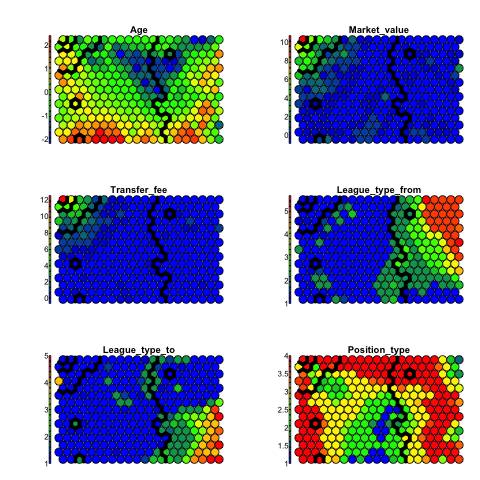
\includegraphics[width=0.6\textwidth]{../figs/transfer_feature_map.png}
    \caption{Plot of each component of trained codebook vectors. 
             Color gradient is blue to green to red. 
             The corresponding labels for position type are 
             \{Goalkeeper, Defender, Midfielder, Forward\} = \{1, 2, 3, 4\}. 
             The corresponding labels for league type are 
             \{Big5, Europe, Americas, Asia/Africa, Big5 B, Other B\} = 
             \{1, 2, 3, 4, 5, 6\}.}
    \label{fig:transfers-variable-plots}
\end{figure}

Looking at the individual variables in Figure~\ref{fig:transfers-variable-plots}, 
we see that high values of transfer fee and market value are clustered towards the top left corner of the grid, 
and that the outliers in these two variables determine 3 out of the 5 clusters. 
Although there is inherent pattern in the age and position type variables, 
they do not seem to influence the clustering of the nodes
since the clustering boundaries do not separate the nodes clearly for either variables.
The last two clusters seem to be determined by a combination of the league type to and from variables. 

\begin{table}[H]
    \centering
    \small
    \begin{tabular}{|lllllll|}
    \hline
        Name & Position & Age & Team\_from & Team\_to & Market\_value & Transfer\_fee \\  \hline
        Neymar & Left Winger &  25 & FC Barcelona & Paris SG  & 100.00 & 222.00  \\ 
        Philippe Coutinho & Attacking Midfield &  25 & Liverpool & FC Barcelona & 90.00 & 125.00 \\ 
        Kylian Mbappé & Right Winger &  19 & Monaco & Paris SG  & 120.00 & 135.00\\ 
        Cristiano Ronaldo & Centre-Forward &  33 & Real Madrid & Juventus & 100.00 & 117.00  \\ 
    \hline
    \end{tabular}
    \caption{Samples in cluster 5 defined by SOM.}
    \label{tab:top_cluster}
\end{table}

Upon closer inspection, 
Table~\ref{tab:top_cluster} shows that the players in cluster 5 
have the highest transfer fees and market values.
This shows that SOM seems to give reasonable clustering behavior
as we see these four highly regarded players placed in a cluster 
very distant from all other nodes.
Similarly, cluster 4 contains truly world-class players.
For example, cluster 4 includes Gareth Bale, Edinson Cavani, \'{A}ngel di Maria, Kevin De Bruyne, and Alisson.
However, while cluster 3 contains notable players, not all are at the very top level.
Some players from cluster 3 are Mateo Kovacic, Granit Xhaka, Memphis Depay, Julian Draxler, and Richarlison.
While we cannot argue that the players in cluster 3 and 4 are significantly of a lower level 
than the ones in cluster 5, 
it is, nonetheless, noteworthy of how SOM selects the boundaries
and that the result is reasonable.

